High level description of the problem with no math. \todonote

\subsection{Formal Problem Statement}

At each time $t$, an arrival is drawn from a set of $n$ types with some known distribution.
Each type $j$ has a random reward drawn from the set $\crl{0,r_{j1},r_{j2}}$; we must make a decision after the type is revealed, but before observing the realized reward.
More precisely, type $j$ is associated with values $r_{j1},r_{j2}>0$ and probabilities $q_{j1},q_{j2}\in[0,1]$ such that $q_{j1}+q_{j2}\leq 1$.
The reward of a type $j$ is $r_{jk}$ with probability $q_{jk}$, $k\in\crl{0,1,2}$, where $r_{j0}\defeq 0$ and $q_{j0}\defeq 1-q_{j1}-q_{j2}$.

The decision-maker is given hiring and probing budgets $\Bh,\Bp\in\N$.
If he chooses to probe an arrival, then he can see the realization of the reward and then decide whether to accept or reject, thus probing protects against low realizations.
He can also choose to accept the arrival without probing, in such case the reward is random, but it does not consume probing budget.

Let us denote the average type $j$ reward by $\bar r_j\defeq r_{j1}q_{j1}+r_{j2}q_{j2}$.
It is instructive to consider extreme cases of $\Bp$.
If $\Bp=\T$, then \onl probes every single arrival, thus the problem corresponds to the multi-secretary with a different arrival distribution.
On the other hand, if $\Bp=0$, then the problem also corresponds to the multi-secretary with each type having reward $r_j$.
If $\Bp$ is any other value, then it is not clear what the interaction between the two budgets is in a good policy.

\subsection{Formulation as a MCDP}
We work in $2\T$ time steps.
At even times, the input reveals the type $j$ and at odd times it reveals the actual realization given probabilities $q_{jk}$
Let us define an \emph{input process} $(\xit)_{t\in[2\T]}$ as a Markov chain in the state space $[n]\cup\crl{(j,k):j\in[n],k=0,1,2}$.
The transition probabilities are given by $P_{j,(j,k)}=q_{jk}$, $P_{(j,k),j'}=p_{j'}$.
For $\xi^{2t-1}=(j,k)$ we define $r(\xi^{2t-1})=r_{jk}$.

The state space (see \cref{fig:probing_states}) can be described as  
\[
\S=\crl{(b_h,b_p),(b_h,b_p,\diamond):b_h,b_p\in\N,\diamond\in \crl{\texttt{a,p,r}}}.
\]
The component $\diamond$ indicates if we are in the accept, probe or reject stage.
There is never a $\diamond$ at times $2t$ and, at $2t-1$, feasible controls are different for distinct $\diamond$.

\begin{figure}
\centering
\scalebox{0.7}{%
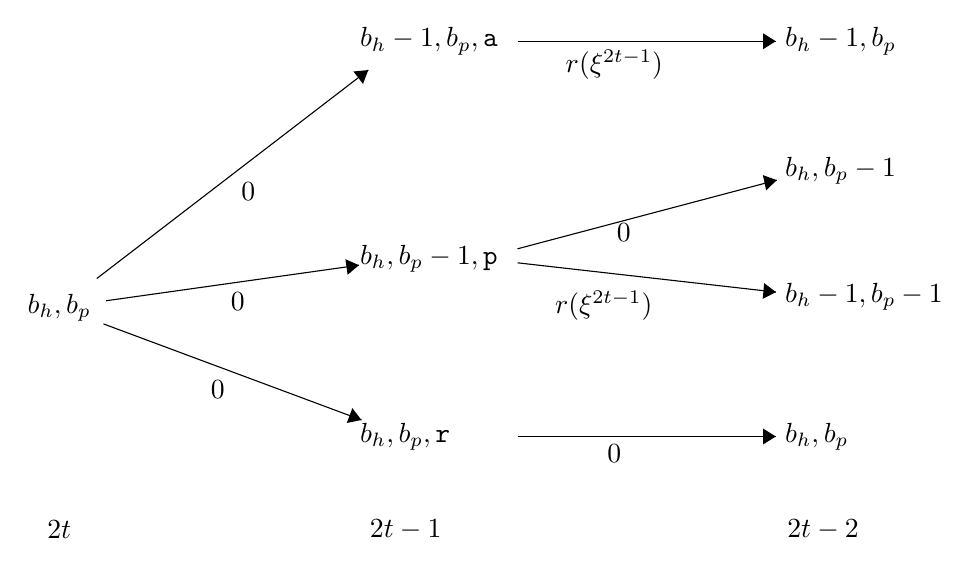
\begin{tikzpicture}[scale=0.2]
\tikzstyle{every node}+=[inner sep=0pt]

\draw (5.9,-25.9) node {$b_h,b_p$};

\draw (5.9,-40) node {$2t$};
\draw (27.9,-40) node {$2t-1$};
\draw (54.4,-40) node {$2t-2$};

\draw (30,-9) node[text width=2cm] {$b_h-1,b_p,\texttt{a}$};
\draw (30,-22.8) node[text width=2cm] {$b_h,b_p-1,\texttt{p}$};
\draw (30,-34.1) node[text width=2cm] {$b_h,b_p,\texttt{r}$};

\draw (57,-9) node[text width=2cm] {$b_h-1,b_p$};
\draw (57,-17.2) node[text width=2cm] {$b_h,b_p-1$};
\draw (57,-34.1) node[text width=2cm] {$b_h,b_p$};
\draw (57,-25.2) node[text width=2cm] {$b_h-1,b_p-1$};


\draw [black] (8.28,-24.07) -- (25.52,-10.83);
\fill [black] (25.52,-10.83) -- (24.58,-10.92) -- (25.19,-11.71);
\draw (17.91,-17.95) node [below] {$0$};
\draw [black] (8.87,-25.48) -- (24.93,-23.22);
\fill [black] (24.93,-23.22) -- (24.07,-22.84) -- (24.21,-23.83);
\draw (17.24,-24.94) node [below] {$0$};
\draw [black] (8.71,-26.95) -- (25.09,-33.05);
\fill [black] (25.09,-33.05) -- (24.51,-32.3) -- (24.16,-33.24);
\draw (15.97,-30.52) node [below] {$0$};

\draw [black] (35,-9) -- (51.4,-9);
\fill [black] (51.4,-9) -- (50.6,-8.5) -- (50.6,-9.5);
\draw (41.15,-9.5) node [below] {$r(\xi^{2t-1})$};
\draw [black] (35,-22.18) -- (51.46,-17.82);
\fill [black] (51.46,-17.82) -- (50.58,-17.5) -- (50.79,-18.47);
\draw (41.75,-20.58) node [below] {$0$};
\draw [black] (35,-23.07) -- (51.41,-24.93);
\fill [black] (51.41,-24.93) -- (50.66,-24.36) -- (50.57,-25.36);
\draw (40.47,-24.83) node [below] {$r(\xi^{2t-1})$};
\draw [black] (35,-34.1) -- (51.4,-34.1);
\fill [black] (51.4,-34.1) -- (50.6,-33.6) -- (50.6,-34.6);
\draw (41.15,-34.6) node [below] {$0$};
\end{tikzpicture}
}
\caption{Transitions for the online probing problem. 
Numbers below the arrows represent the reward of a transition.
At time $2t$ the possible actions are: accept, probe and reject.
At $2t-1$, depending on $\diamond$, we can either accept or reject and $b_h$ may be discounted.
}
\label{fig:probing_states}
\end{figure}


\subsection{Relaxation for Multiple Probing}

For every arrival we decide first whether to probe, reject or accept.
If we decide to probe, then there is a second decision, which uses the new information.
Say we observe type $j$ and $r_{j1}>r_{j2}>0$.
It is obvious that if the realization has zero reward we should reject.
An exchange argument shows that, if probing was optimal, then the value $r_{j1}$ must be accepted.
On the other hand, it is unclear if $r_{j2}$ should be accepted.
We must, therefore, reason about \off's actions at all times, instead of just at even times as before and concluding with structural properties.

Let $\calX\defeq\Rp^{7n}$ be the space for the decision variables.
In \cref{eq:probing_lp} we present a LP which will be the building block for our relaxation.
Note that, by definition, if $t$ is odd, $Z_j(t)=Z_j(t+1)-\In{\xi^{t+1}=j}$.

\begin{equation}\label{eq:probing_lp}
\begin{array}{rrll}
(P[t,b]) \; \max & \multicolumn{3}{l}{\sum_{j,k}r_{jk}x_{jka}+ \sum_j \bar r_jx_{ja}} \\
\text{s.t.}& \sum_{j,k}x_{jka}+\sum_jx_{ja} &\leq b_h  \\
&  \sum_j x_{jp} & \leq b_p   \\
&  x_{ja} +x_{jp} + x_{jr}&= Z_j(t)  & \forall j \\
& x_{jka} +x_{jkr} &= q_{jk}x_{jp} &  \forall j,k\\ 
& x&\in\calX.
\end{array}
\end{equation}

The LP in \cref{eq:probing_lp} can be interpreted as follows...\todonote

We are ready to parse the relaxation in \cref{eq:probing_relax}.
Recall that a state is of the form $s=(b_h,b_p,\diamond)$ with $\diamond\in \crl{\texttt{a},\texttt{p},\texttt{r},\varnothing}$, where $\diamond=\varnothing$ for even times.
The relaxation can be interpreted as giving \off the power to run a two-stage DP, where the value function is given by the corresponding LP.... \todonote
\begin{equation}\label{eq:probing_relax}
\varphi(t,s,\xit) = \left\{ 
\begin{array}{ll}
vP[t,b] & \diamond=\varnothing \\ 
vP[t-1,b] & \diamond = \texttt{r} \\ 
r_{\xit}+vP[t-1,b] & \diamond = \texttt{a} \\ 
\max\crl{r_{\xit}+vP[t-1,b-e_h],vP[t-1,Z,b]} & \diamond = \texttt{p}
\end{array} 
\right.
\end{equation}

We proceed to show that the relaxation satisfies the two conditions for the relaxed Bellman equations in \cref{def:relaxed_bellman}.
In \cref{lem:probing_initial} we show the initial condition and in \cref{lem:probing_ineq} the probabilistic inequality.


\anote{This is the proof for the active/inactive case. Need to update it}
\begin{lemma}\label[lemma]{lem:probing_initial}
For any $b_h,b_p\in\N$, $t\in[\T]$ and realization $Z$ of arrivals, $\voff(2T,b) \leq \varphi(2\T,(b,\varnothing),\xi^{2\T})$ 
\end{lemma}
\begin{proof}
Consider any policy for \off which determines when to probe, accept or reject.
The policy induces a random trajectory, which is determined by the realization of the Bernoulli variables, not the arrivals, since the later are given.
Define the following random variables, counting the number of times in which a type $j$: was probed, denoted $Y_j$; was accepted without probing, $X_{ja}$; and was accepted after probing, $X_{jp}$.
Finally, let $Y_{j}^+,X_{ja}^+$ be the number of active from among those probed or accepted, respectively.
We assume w.l.o.g.\ that, among the probed elements, \off takes only active ones.

Our aim is to argue that, replacing the aforementioned r.v.\ with their expectations, yields a feasible solution to $(P^\star)$.
It holds $\voff(t,b_h,b_p) = \E[\sum_j r_j(X_{jp}+X_{ja}^+)]$ and $\E[X_{ja}^+|X_{ja}]=q_jX_{ja}$, thus
\[
\voff(t,b_h,b_p) = \sum_jr_j(\E[X_{jp}]+q_j\E[X_{ja}]).
\] 

With the exception of the constraint $x_{jp}\leq q_jy_j$, $X_{ja},Y_j,X_{jp}$ satisfy a.s.\ all the constraints of $(P^\star)$, hence their expectations do too.
Observe that $X_{jp}\leq Y_{j}^+$ and $\E[Y_j^+]=q_j\E[Y_j]$, thus $\E[X_{jp}]\leq q_j\E[Y_j]$.
To summarize, $\voff(t,b_h,b_p)$ equals the value of the feasible solution given by the expectations, so $v(P^\star)$ can be only larger.
\end{proof}

\begin{lemma}\label[lemma]{lem:probing_ineq}
Let $\bar X\in\calX$ be a maximizer of $(P[t,b])$ for $t$ even.
Say $\xit=i$, then, at time $t$, \off is satisfied with the following actions:
\begin{enumerate}
\item Accept if $\bar X_{ia}\geq 1$
\item Reject $\bar X_{ir} \geq 1$
\item Probe if $\bar X_{ip}\geq 1$ and then accept $(i,k)$ if $\bar X_{(i,k)a}\geq 1$ or reject if $\bar X_{(i,k)r}\geq 1$
\end{enumerate}
\end{lemma}
\begin{proof}
We need to show the probabilistic inequality
\[
\varphi(t,s,\xit) \leq \max_{u\in\U}\crl{R(s,\xit,u)+\E_{\xi^{t-1}}[\varphi(t-1,\Tr(s,\xit,u),\xi^{t-1})|\xit]} \quad \forall \omega\in\calB(t,s).
\]
The set $\calB(t,s)$ is defined as the $\omega\in\Omega$ such that at least one of the conditions (1),(2) or (3) are satisfied.
Observe that, since $t$ is even, the instant reward $R(s,\xit,u)$ is zero.
In cases (1) and (2) is easy to verify the probabilistic inequality.
For case (3) we need to introduce some notation.
Let $\vec q_{j}\in\R^{2n}$ be a vector with value $q_{jk}$ in components $(j,k)$, $k=1,2$, and zero otherwise.
Similarly, let $\vec 1_{(j,k)}\in\R^{2n}$ have value $1$ in the single component $(j,k)$ and zero otherwise.
The following LP is the same as in \cref{eq:probing_lp}, but has an extra parameter to facilitate the analysis.
In particular, $vP[t,b]=v\bar P[t,b,0]$.

\begin{equation}
\begin{array}{rrll}
(\bar P[t,b,y]) \; \max & \multicolumn{3}{l}{\sum_{j,k}r_{jk}x_{jka}+ \sum_j \bar r_jx_{ja}} \\
\text{s.t.}& \sum_{j,k}x_{jka}+\sum_jx_{ja} &\leq b_h  \\
&  \sum_j x_{jp} & \leq b_p   \\
&  x_{ja} +x_{jp} +x_{jr} & \leq Z_j(t)  & \forall j \\
& x_{jka} +x_{jkr} &= q_{jk}x_{jp}+y &  \forall j,k.
\end{array}
\end{equation}

In case (3) we assume that the following holds: for every $k$, either $\bar X_{ika}\geq 1$ or $\bar X_{ikr}\geq 1$.
In other words, the LP wants to either fully reject one item or fully accept it.
With this assumption, denoting $I\defeq \In{\bar X(\xi^{t-1},a)\geq 1} $, we can write the following  a.s.\ equality (recall that $\xi^{t-1}$ is unknown at $t$)
\[
vP[t,b] = r_{\xi^{t-1}}I + v\bar P[t-1,b-e_p-e_hI,\vec q_{\xit}-\vec 1_{\xi^{t-1}}].
\]

In words, since $\bar X_{ip}\geq 1$, we can discount one in this variable when solving the LP, which reduces $b_p$ by $1$, $Z_j(t)$ by one and increases $y$ from $0$ to $\vec q_{i}$.
On the other hand, since either $\bar X_{ika}\geq 1$ or $\bar X_{ikr}\geq 1$, we can always discount $1$ from a single component $(i,k)$, which decreases $y$ by one in the corresponding component.
Finally, the indicators enforce that discounting from accept variables $\bar X_{ika}$ is preferable.

Now we can take expectations $\E[\cdot |\xit]$ and use Jensen's Inequality in only the variable $y$ of $\bar P$ as follows.
\begin{align*}
vP[t,b] &= \E[r_{\xi^{t-1}}I + v\bar P[t-1,b-e_p-e_hI,\vec q_{\xit}-\vec 1_{\xi^{t-1}}] |\xit] \\
&\leq \E[r_{\xi^{t-1}}I+ v\bar P[t-1,b-e_p-e_hI, 0] |\xit].
\end{align*}
Finally, since one of the options upper bounds $vP[t,b]$, surely the maximum does too, which is $\varphi(t-1,(b-e_p,\texttt{p}),\xi^{t-1})$.

\anote{What's going on is just a technical challenge. When we decide to probe at $t$, the right hand side does not go down by the same amount as the fluid does.
We need to justify that, in expectation you get a problem with a right hand side working in your favour.}
\end{proof}

Now we can invoke \cref{prop:relaxed_bellman} to conclude that \off is satisfied following the maximizers of our relaxation as long as fractional variables $(0,1)$ can be avoided.
Finally, we show how our policy approximates the solutions... \todonote

Consider the policy that, at even times solves $(P[t,\Bt])$, but with $Z(t)$ replaced by $\mu(t)\defeq \E[Z(t)]$ to get a solution $\Xt$.
Say $\xit=i$ is the current arrival.
If $\Xt_{ia}\geq \mu_{i}(t)/3$, the arrival is accepted.
Else if $\Xt_{ip} \geq \mu_i(t)/3$, the arrival is probed and then accepted contingent on $\Xt_{\xi^{t-1},a}\geq q_{\xi^{t-1}}\bar X_{ip}/2$.
Else, the arrival is rejected.

\begin{theorem}
The policy has regret bounded by a constant that depends on $n,q$ and the distribution of $Z(t)$ only.
\end{theorem}
\begin{proof}
Let $\Xts$ be a solution to $P[t,b]$.
In virtue of \cref{lem:probing_ineq}, if the policy accepts or rejects, the error is bounded by
\[
\Pr[\Xts_{i\diamond}<1|\Xt_{i\diamond}\geq \mu_i(t)/3], \quad \diamond=\texttt{a},\texttt{r}.
\]

If the policy probes, the error is bounded by the following, where $\diamond$ is the action with largest value between the variables $\Xt{\xi^{t-1},a},\Xt{\xi^{t-1},r}$.
\[
\Pr[\Xts_{ip}<1 \text{ or } \Xts_{\xi^{t-1},\diamond}<1|\Xt_{ip}\geq \mu_i(t)/3, \Xt_{\xi^{t-1},\diamond}\geq q_{\xi^{t-1}}\mu_i(t)/6 ]
\]

\anote{Now we can finish with the Lipschitz argument.
I'm not a big fan of it, because I'm still not sure if that's the best way to go about it, but it does abstract away all the technicalities in the deviations.

The exact regret bound would depend on the Lipschitz constant. I'm not sure how valuable it is to bound it more precisely.
}
\end{proof}